\documentclass[10pt,twocolumn]{article}
\usepackage{amsmath}
\usepackage{amsfonts}
\usepackage{graphicx}
\usepackage{mathtools}
\usepackage{fullpage}
\usepackage{float}
\usepackage{color, soul}

\begin{document}
\title{6.867 HW2: Binary Classification Methods}
\maketitle
When making predictions and models, sometimes we would rather have discrete labels instead of continuous values. For example, if we were looking exam results, we might only care if students pass or fail. Alternatively, we may want to study electricity patterns, and at any given time lights can either be on or off. This idea of discrete labels is known as classification and in the case that there are only two options, binary classification. For the following work, we will consider the class labels $\{-1, +1\}$. 

\section{Logistic Regression}
 
 The first method we will use to implement binary classification will be logistic regression. The use of logistic functions, specifically the sigmoid, allow us to map continuous values of input values to a corresponding probability between 0 and 1, which then can be used to select a discrete label. Considering the maximum likelihood estimation, logistic regression can be written as 
 \begin{equation}
 \textrm{MLE}(w)= \sum_{i=1}^{n} \textrm{log}(1+e^{-y^{(i)}w^T \Phi(x^{(i)})})
 \end{equation}
 Where $w$ are the weights defining our model, $x(i), y(i)$ given data points, and $\Phi$ the basis functions from which we construct our model. Letting the basis function be a simple linear formulation, $\Phi(x)= \begin{bmatrix} 1 & x _1 & x_2 & ... \end{bmatrix}^T$, the above equation can be simplified as 
 \begin{equation}
\textrm{ NNL}(w)= \sum_{i=1}^{n}\textrm{ log}(1+e^{-y^{(i)}(w_0+w^Tx^{(i)})})
 \end{equation}
 However to prevent overfitting, we also want to introduce a regularization term into the logistic regression error function. Specifically we will consider a quadratic regularizer, which results in the finalized error function, 
 \begin{equation}
 E_{LR}(w)= \textrm{NNL}(w) +\lambda w^Tw
 \end{equation}
 Unlike some of the regression formulations we looked at last time, such as ridge or linear, there is no closed from solution to minimizing the error. Thus, we must employ optimization methods to select the correct weights. As far as optimization methods,we used a simple gradient descent. 
 
 Once weights are calculated from minimizing the error on the training data our classifier is simply defined as, 
 \begin{equation}
 h=\textrm{sign}(w^Tx +w_0)
 \end{equation}
 Which simply creates a hyperplane in which for any input, $x$. This classification returns -1 if $w^Tx+w_0<0$ and +1 if $w^Tx\geq 0$. The boundary decision is marked by $.5= \sigma (w^Tx)$ and is shown below for the case where there is no regularizer. 
 

 
 \begin{figure}[H]
\center
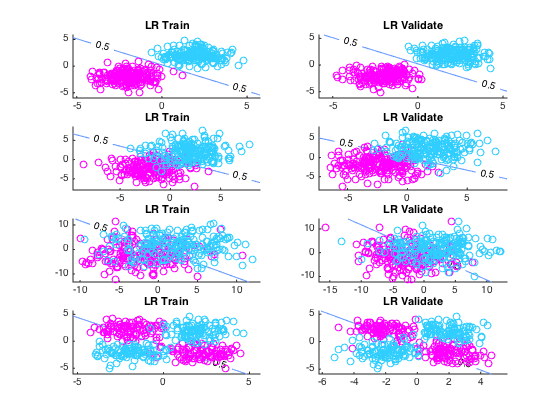
\includegraphics[scale =.4]{p1lambda0.png}
\caption{Labelled test and validation data for stdev1,stdev2, stdev4 and nonsep data sets. Also shown is the decision boundary }
\end{figure}
 
 Also considered was the error from mislabelled points, which was calculated for both the test and validation sets. Of course, the more easily separable the data, the lower the error. These results are shown in Table \ref{LR error}

As the magnitude of w increases the steepness of the hyperplane increases.  If $w$ goes to $ \infty$ the separator becomes a step function. The regularizer helps to limit this by penalizing the magnitude of the weights. It also helps prevent overfitting. So as $\lambda$ is increased the training error might increase since the cost is less influenced on the data error, NLL, and more influenced by the weights. 


We tested this logistic regression for $\lambda= \{0, 10, 1000\}$ and for the clearly separable and non separable case, there was no effect. For the stdev2, and stdev4 cases the training error increases but the validation error decreases. These results are shown in Table \ref{LR error}

 \begin{table}
 \caption{ Training and Validation Errors for different regularizers, $\lambda$}
  \begin{tabular}{ | c | c | c | c |}
 \hline
 dataset &$ \lambda=0 $& $\lambda=10$ & $\lambda=1000$ \\ \hline 
 stdev1 & [0,0] & [0,0] & [0,0] \\ \hline
 stdev2 & [36, 29] & [36,30] & [41, 26] \\ \hline
 stdev4 & [105, 99] & [105, 99] & [106, 98] \\ \hline 
 nonsep & [239, 247] & [243, 247] & [233, 228] \\ \hline
 \end{tabular}
 \label{LR error}
\end{table}
 
 
 
 \section{Support Vector Machine}
 
 Another implementation method of binary classification is the Support Vector Machine. In this classification method, we seek to divide the data into the different classifications with a clear a gap as possible. This gap or margin is defined as support vectors and takes advantage of the hinge loss.  The simplest form of SVM, the primal hard form, is expressed as 

 \begin{equation}
\min_w ||w||^2
\end{equation}
\begin{equation}
s.t. \: \forall i, y^{(i)}w^T x^{(i)} \geq 1 
 \end{equation}
    
 The hard form of SVM does not allow any leeway on the constraints, making it impossible to create a model if the data is not linearly separable. To increase the capability of the SVM, the soft SVM, includes a slack variable, $\xi$, For the straight forward primal form of soft SVM applied to the linear case,  $\Phi(x)= \begin{bmatrix} 1 & x _1 & x_2 & ... \end{bmatrix}^T$ , the overall objective once combined with corresponding constraint is thus
 \begin{equation}
 \min_{w, w_0} (\frac{1}{2} ||w||^2 + C \sum_{i=1}^n \xi_i)
 \end{equation}
 \begin{equation}
 s.t. \: y^{(i)}(w^Tx^{(i)} + w_0) \geq 1 -\xi_i
 \end{equation}   
 \begin{equation}
 \xi_i \geq 0
 \end{equation}
    
    
This formulation is not ideal, instead we translate this to the dual form which using an auxiliary variable, $\alpha$ to rewrite the SVM as a maximization and clearly shows the optimization as a maximum margin. 

\begin{equation}
\max_{\alpha \in \mathbb{R}^n} ( \sum_{i=1}^n \alpha_i - \frac{1}{2} \sum_{i=1}^n \sum_{j=1}^n \alpha_i \alpha_j y^{(i)} y^{(j)} (x^{(i)})^T x^{(j)})
\end{equation}
\begin{equation}
s.t. \: 0 \leq \alpha_i \leq C
\end{equation}
\begin{equation}
\sum_{i=1}^n \alpha_i y^{(i)} =0
\end{equation}

Instead of optimizing over the weights explicitly, we optimize over $\alpha$ from which the weights can be directly calculated as 
\begin{equation}
w= \sum_{i=1}^n \alpha_i y^{(i)}x^{(i)}
\end{equation}  
\begin{equation}
w_0= \frac{1}{M} ( \sum_{j \in M} y^{(j)} - \sum_{i \in S} \alpha_i y^{(i)}(x^{(j)})^Tx^{(i)})
\end{equation}

Where $S$ is the set of support vectors, $S=\{i : 0 < \alpha_i \leq C \}$ and $M = \{i : 0 < \alpha_i < C \}$. However since there is some numerical residual resulting from the optimizations of $\alpha$ that won't exactly equal 0 or C we will consider the small tolerance, $\epsilon= 10^-5$ so that  $S=\{i : \epsilon < \alpha_i \leq C-\epsilon \}$ and the same for M.

The MATLAB function $quadprog$ minimizes the function $1/2 x^T H x + f^T x$ with the constraints $Ax <= b$ and $A_{eq}x = b_{eq}$. For this portion, we set 
\begin{gather*}
H = diag(y)xx^Tdiag(y)\\
f = -\mathbf{1} _{n \; \textrm{x} \; 1}\\
A = \begin{bmatrix}-I_{n \; \textrm{x} \; n} \\ I_{n \; \textrm{x} \; n} \end{bmatrix}\\
b = \begin{bmatrix}  \mathbf{0} _{n \; \textrm{x} \; 1}\\  \mathbf{C} _{n \; \textrm{x} \; 1} \end{bmatrix}\\
A_{eq} = y^T\\
b_{eq} = 0\\
\end{gather*}
Where the bold terms indicate matrixes of constant value of size denoted by the subscript and $n$ is the length of the input data. 


This yielded $\alpha = [0.5306, 0.0000, 0.3673, 0.1633]$ for the input $x = [1,2 ; 2,2 ; 0,0 ; -2,3]$ and $y = [1,1,-1,-1]$. This makes intuitive sense because the non support vector, (2,2), has an $\alpha$ value of 0.


This SVM was applied to the data from problem 1, stdev1,stdev2, stdev4 and nonsep, test and validation sets. Initially we looked at the case where $C =1$. The plotted results are shown in Fig. \ref{SVM C1} and the corresponding errors in Table \ref{SVM C1 T}. 


 \begin{figure}[H]
\center
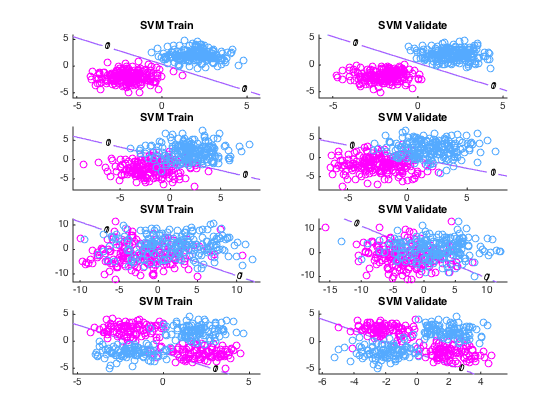
\includegraphics[scale =.4]{p2C1.png}
\caption{Labelled test and validation data for stdev1,stdev2, stdev4 and nonsep data sets when $C=1$. Also shown is the decision boundary }
\label{SVM C1}
\end{figure}

 \begin{table}
 \caption{ Training and Validation Errors for $C=1$}
  \begin{tabular}{ | c | c | c | }
 \hline
 dataset & Test Error & Validation Error  \\ \hline 
 stdev1 & 0 & 0 \\ \hline
 stdev2 & 38 & 32 \\ \hline
 stdev4 & 102 & 94 \\ \hline 
 nonsep & 118 & 121 \\ \hline
 \end{tabular}
 \label{SVM C1 T}
\end{table}


Clearly the more overlapped the data is the more errors the classifier makes. However comparing with the results from Table \ref{LR error}, the SVM implemented here outperforms our logistic regression algorithm for stdev4 (102, 94 vs 105, 99 ) and nonsep (118, 121 vs  243,247). 

\subsection*{Kernels}

The multiplication $x^Tx$ appears in multiple locations for out SVM calculations, both in  the optimization of the $\alpha_i$ and in the calculation of $w_0$. The idea of kernel trick is that we can rewrite anything the terms there as a kernel function, $k(x,z)$ replacing any terms that can be expressed as inner products. Using this formulation the SVM can be written as 

\begin{equation}
\max_{\alpha \in \mathbb{R}^n} ( \sum_{i=1}^n \alpha_i - \frac{1}{2} \sum_{i=1}^n \sum_{j=1}^n \alpha_i \alpha_j y^{(i)} y^{(j)} k(x^{(i)},x^{(j)})
\end{equation}
\begin{equation}
s.t. \: 0 \leq \alpha_i \leq C
\end{equation}
\begin{equation}
\sum_{i=1}^n \alpha_i y^{(i)} =0
\end{equation}
\begin{equation}
w= \sum_{i=1}^n \alpha_i y^{(i)}x^{(i)}
\end{equation}  
\begin{equation}
w_0= \frac{1}{M} ( \sum_{j \in M} y^{(j)} - \sum_{i \in S} \alpha_i y^{(i)}k(x^{(j)},x^{(i)})
\end{equation}

With the decision boundary, 

\begin{equation}
\sum_{i:\alpha_i > 0} \alpha_i y^{(i)}k(x^{(i)}, x) + w_0 = 0.
\end{equation}

 More importantly kernels are adaptable to a range of basis functions. It can be used for anything that can be written as an inner product. In particular we chose to look at the Gaussian Kernel
 \begin{equation}
 k(x,z)= \textrm{exp}(-\frac{1}{2\sigma^2} ||x - z||_2^2)
\end{equation}

Where $\sigma$ is the bandwidth.

Trying the Guassian Kernel on the data sets already mention, with $C= .01, \sigma =.1$ the following results were obtained

 \begin{figure}[H]
\center
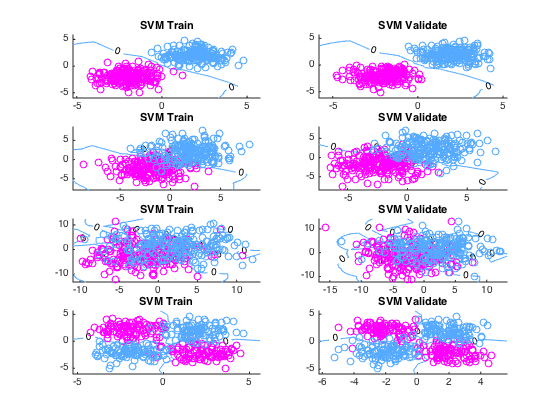
\includegraphics[scale =.4]{Cpt01BWpt1.png}
\caption{Labelled test and validation data for stdev1,stdev2, stdev4 and nonsep data sets when $C=.01, \sigma =.1$ with Gaussian Kernel. Also shown is the decision boundary }
\label{SVM Gauss C01}
\end{figure}
 
 Increasing $\sigma$ leads to Fig. \ref{SVM Gauss C10}. Where one can see that the decision boundary has become more linear
 \begin{figure}[H]
\center
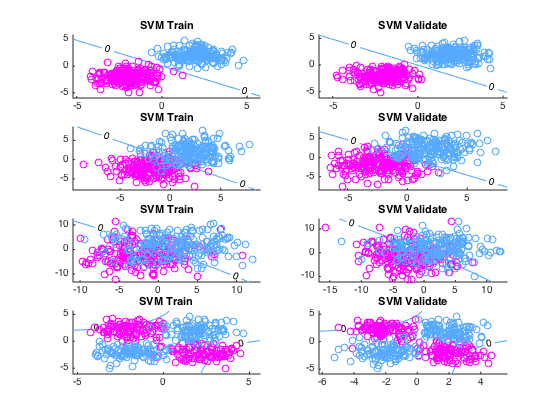
\includegraphics[scale =.4]{Cpt01BW10.png}
\caption{Labelled test and validation data for stdev1,stdev2, stdev4 and nonsep data sets when $C=.01, \sigma =10$ with Gaussian Kernel. Also shown is the decision boundary }
\label{SVM Gauss C10}
\end{figure}

As shown in Fig. \ref{SVM Gauss C01} The gaussian kernel performs a lot better on the non separable data. 
       
 Using a constant value of $\sigma=.1$ we investigated the effect of changing $C$ on the geometric margin, $\frac{1}{||w||}$ and the number of support vectors, $S$. In particular we considered $C= \{.01, .1, 1, 10, 100 \}$
 and the  results are shown in Tables \ref{SVM Gauss Marg} and \ref{SVM Gauss S}
 

When C increases,the geometric margin decreases as does the number of support vectors. This is because the slack variables are being penalized more and more resulting in smaller margins. However when C becomes too large, the problem becomes hard SVM and it may not be possible to separate the data. 

 \begin{table}
 \tiny
 \caption{ Geometric Margin for varying $C$}
  \begin{tabular}{ | c | c | c | c | c | c| }
 \hline
 dataset & $C=.01$ & $C=.1$ & $C=1 $ & $C=10$ & $C=100$   \\ \hline 
 stdev1 & .089 &  .013 & 8.08 $\cdot 10^-3$ & 2.85 $\cdot 10^-3$ & 3.49 $\cdot 10^-4$ \\ \hline
 stdev2 & .088 & .009 & 2.40 $\cdot 10^-3$  & 3.72 $\cdot 10^-4$ & 4.01 $\cdot 10^-5$\\ \hline
 stdev4 & .096 & .010 & 1.71 $\cdot 10^-3$  & 3.25 $\cdot 10^-4$ & 3.57 $\cdot 10^-5$\\ \hline 
 nonsep & 3.03 & .300 & 2.78 $\cdot 10^-2$  &  3.11 $\cdot 10^-3$ & 1.59 $\cdot 10^-4$\\ \hline
 \end{tabular}
 \label{SVM Gauss Marg}
\end{table}

\begin{table}
 \scriptsize
 \caption{ Number of Support Vectors for varying $C$}
  \begin{tabular}{ | c | c | c | c | c | c| }
 \hline
 dataset & $C=.01$ & $C=.1$ & $C=1 $ & $C=10$ & $C=100$   \\ \hline 
 stdev1 & 400  &  400 & 396 & 388 & 364  \\ \hline
 stdev2 & 400 & 400 & 386  & 346 & 302 \\ \hline
 stdev4 & 400 & 392 & 369 & 294 & 263 \\ \hline 
 nonsep & 400 & 398 & 375  &  332 & 307 \\ \hline
 \end{tabular}
 \label{SVM Gauss S}
\end{table}

\section{Titanic Dataset}

In this section we use the classifiers developed above to make predictions of survival for the Titanic dataset provided by Kaggle. The dataset is divided into train, test, and validation subsets, which will be used to train and evaluate the performance of the classifiers. Each row of the data represents the information of one person aboard the Titanic, including important information such as sex, name, age, and more, along with whether they survived. We are tasked with producing a classifier that will be able to accurately predict whether a passenger survived given some of their background information.

\subsection*{Logistic Regression}

We first use a logistic regression classifier. We chose not to use our implementation of gradient descent, but to instead use fminunc. This will learn the weights for each of the 11 features using the training dataset. Using these learned weights, we will to be able to make predictions about whether future cases lived or died given their information. This processes was performed on the validation set. Table 5 shows the resulting error and most predictive feature for different values of $\lambda$ on the validation set.

\begin{table}
 \caption{Logistic regression on Titanic dataset}
  \begin{tabular}{ | c | c | c | c |}
 \hline
 $\lambda$ & Test Error \% & Validation Error \% & Most Important  \\ \hline 
 10 & 21.5 & 24.2 & Class  \\ \hline
 1 & 16.0 & 20.2 & Sex  \\ \hline
 0.5 & 16.5 & 20.4 & Sex \\ \hline
 0.1 & 17.0 & 20.6 & Sex \\ \hline 
 0.01 & 17.0 & 20.4 & Sex \\ \hline
 \end{tabular}
 \label{SVM C1 T}
\end{table}
      
\subsection*{Support Vector Machine}

In this section we evaluate the performance of a SVM classifier. We start by training the SVM weights using the provided training dataset, similar to the logistic regression example. Once we have the fitted weighs, we can use the SVM to classify new examples, then evaluate the performance using the labels. Table 6 shows the resulting errors on the validation and training set, along with the most predictive feature for different values of $C$ .

\begin{table}
 \caption{SVM on Titanic dataset}
  \begin{tabular}{ | c | c | c | c |}
 \hline
 $C$ & Test Error \% & Validation Error \% & Most Important  \\ \hline 
 10 &  19.6 & 21.1 &  Sex \\ \hline
 1 & 19.5 & 21.0 & Sex  \\ \hline
 0.5 & 19.7 & 21.3 & Sex \\ \hline
 0.1 & 19.9 & 21.8 & Sex  \\ \hline 
 0.01 & 32.5 & 31.6 & Sex \\ \hline
 \end{tabular}
 \label{SVM C1 T}
\end{table}

\subsection*{Comparison}

As you can see, both the SVM and logistic regression classifiers are able to predict with similar accuracies, both with peak performances around 20\% error. The logistic regression classifier took longer to train, but in the end the performances are similar. In both cases, the most indicative feature of survival is the sex of the passenger. A female was much more likely to survive than a male passenger. This seems to be in line with what history says, as women were the first to be boarded on the life boats as the Titanic began to sink.

There were other important features which determined the survival rate of a passenger. The next two most important for both classifiers was a passenger's class and age. In general, these features were a little less than half as indicative as sex. On average, the weight vector corresponding to class and age was around .7, while the average weight of sex was around 1.8. From the data, it seems that the highest probability of survival belonged to a young, first class, woman. This can even be seen in the final scenes of the Titanic movie, as Rose (a female) survives the crash, but Jake (male) is unable to survive the cold waters of the Atlantic ocean. 
      
\end{document}
